\begin{figure}[hbt!]
    \begin{subfigure}[b]{0.5\textwidth}
        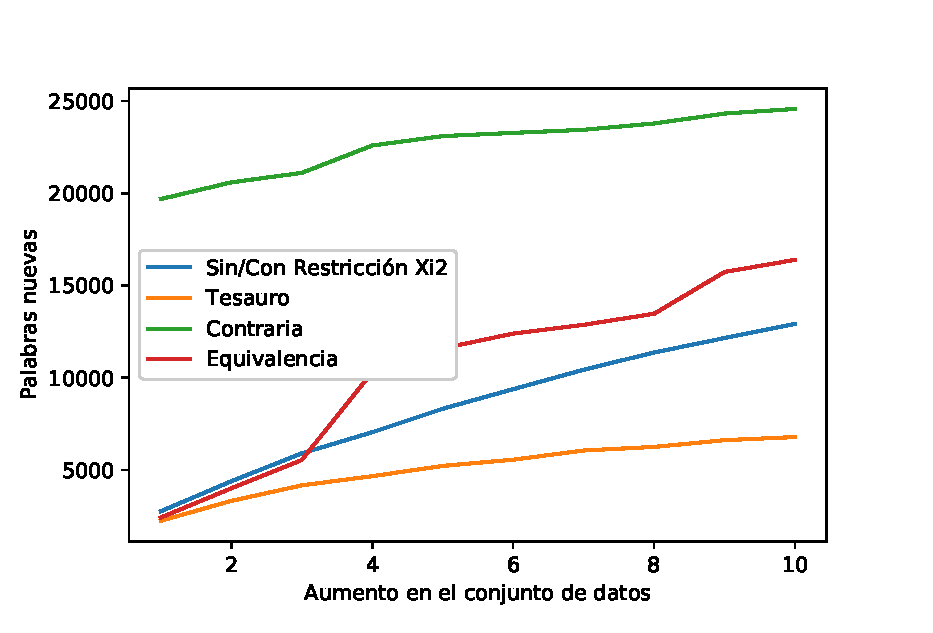
\includegraphics[width=\textwidth]{sections/figures/pos_2018.eps}
        \caption{Depresión 2018: Clase positiva}
    \end{subfigure}
    \hfill
    \begin{subfigure}[b]{0.5\textwidth}
        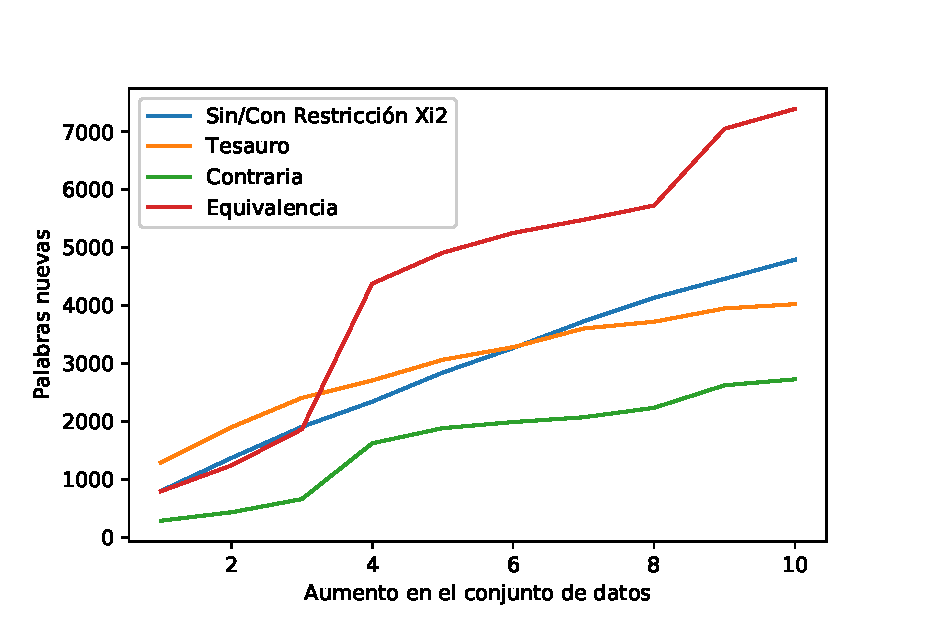
\includegraphics[width=\textwidth]{sections/figures/both2018.eps}
        \caption{Depresión 2018: Ambas clases}
    \end{subfigure}
    \hfill
    \begin{subfigure}[b]{0.5\textwidth}
        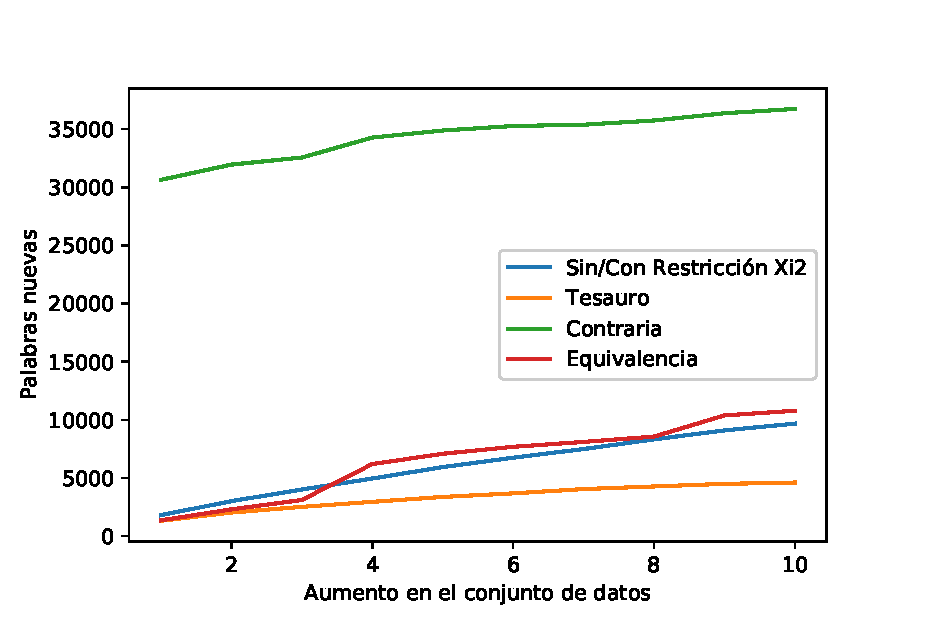
\includegraphics[width=\textwidth]{sections/figures/pos2019.eps}
        \caption{Depresión 2019: Clase positiva}
    \end{subfigure}
    \hfill
    \begin{subfigure}[b]{0.5\textwidth}
        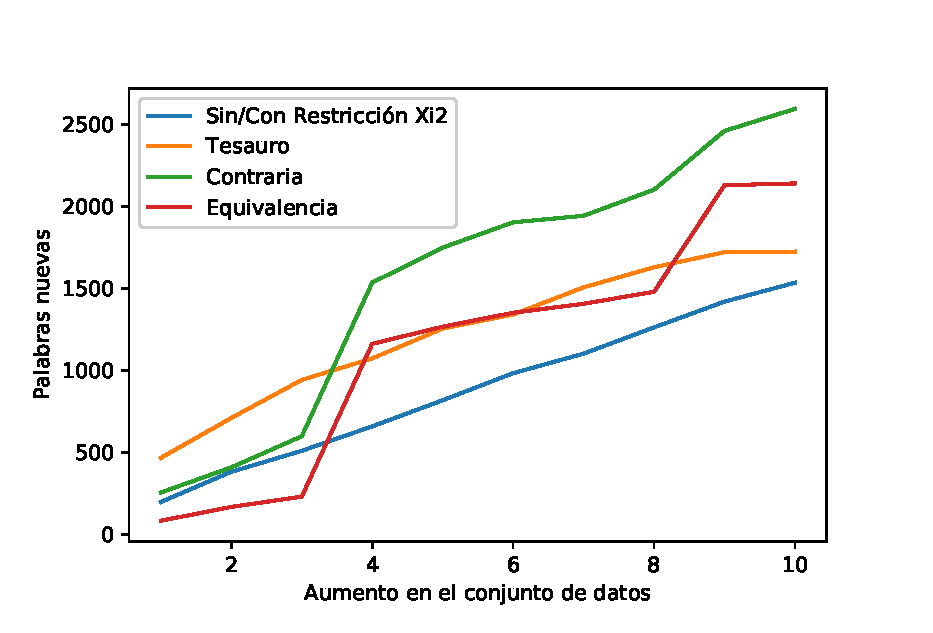
\includegraphics[width=\textwidth]{sections/figures/both2019.eps}
        \caption{Depresión 2019: Ambas clases}
    \end{subfigure}
    
    \begin{subfigure}[b]{0.5\textwidth}
        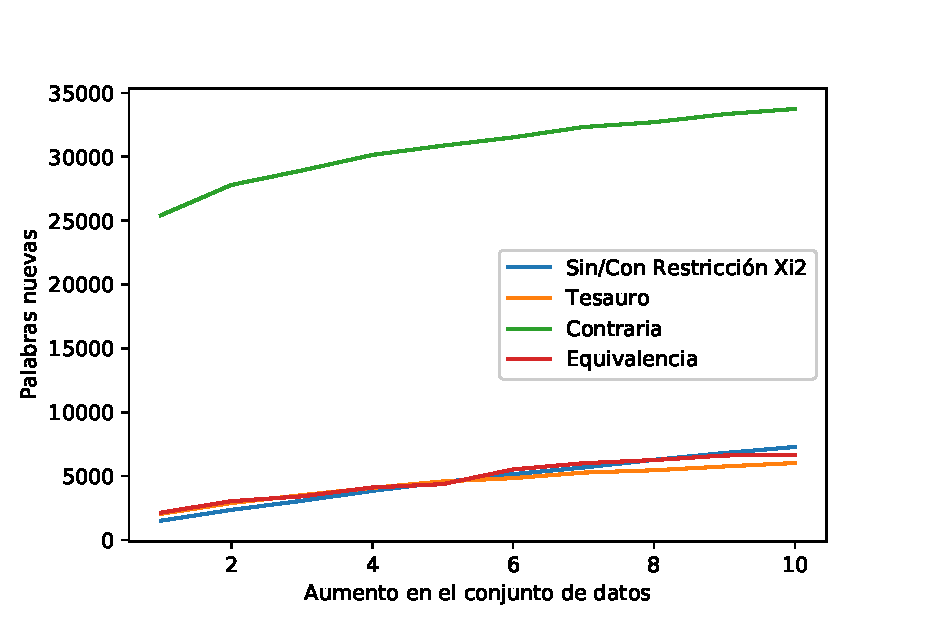
\includegraphics[width=\textwidth]{sections/figures/pos_anox.eps}
        \caption{Anorexia: Clase positiva}
    \end{subfigure}
    \hfill
    \begin{subfigure}[b]{0.5\textwidth}
        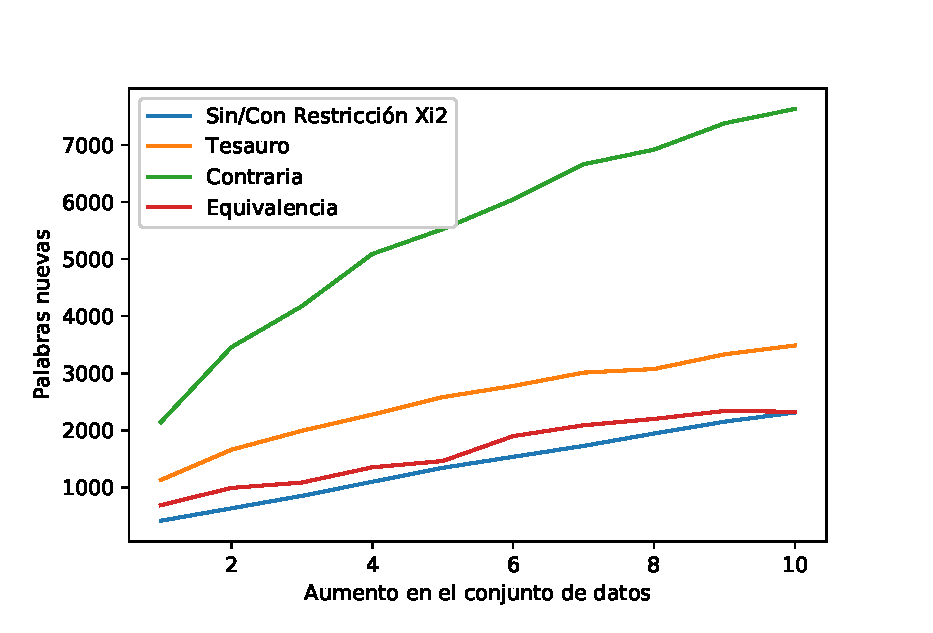
\includegraphics[width=\textwidth]{sections/figures/both_anox.eps}
        \caption{Anorexia: Ambas clases}
    \end{subfigure}
    
    
    \caption{Relación entre el aumento de datos y el vocabulario nuevo agregado.}
    \label{fig:aumento_vocab_dep}
\end{figure}